\documentclass{standalone}
%
\usepackage{tikz}
\usetikzlibrary{backgrounds,shapes.callouts}
\usepackage{tkz-euclide}
%
\usepackage{xcolor}
\definecolor{space}{HTML}{1F2C4E}
\definecolor{earth}{HTML}{0089FA}
\definecolor{dida}{HTML}{FFDE00}
\definecolor{title}{HTML}{FBA706}
\definecolor{moon}{HTML}{AFAFAF}
\definecolor{craterm}{HTML}{616060}
\definecolor{linem}{HTML}{DBDBDB}
%
\usepackage{fontspec}
\setmainfont{Open Dyslexic}
%
\title{Itinerario di un'astrofisica}
\begin{document}
	\tikzset{
		notice/.style  = { draw, ellipse callout, callout relative pointer={#1} },
	}
	\begin{tikzpicture}
		\draw [use as bounding box,color=white] (0,15.5) -| (30,15.5) |- (30,-128.5) -| (0,-128.5);
		%title
		\draw [black,ultra thick,fill=title] (-1,7) rectangle (31,15);
		\node (example-textwidth-2) [right, align=center, text width=30cm, color=black, font=\fontsize{90pt}{91pt}\selectfont] at (0,11) {Itinerario di un'astrofisica};
		% arcetri
		\begin{scope}[shift={(0,-8)}]
			\node at (15,0) {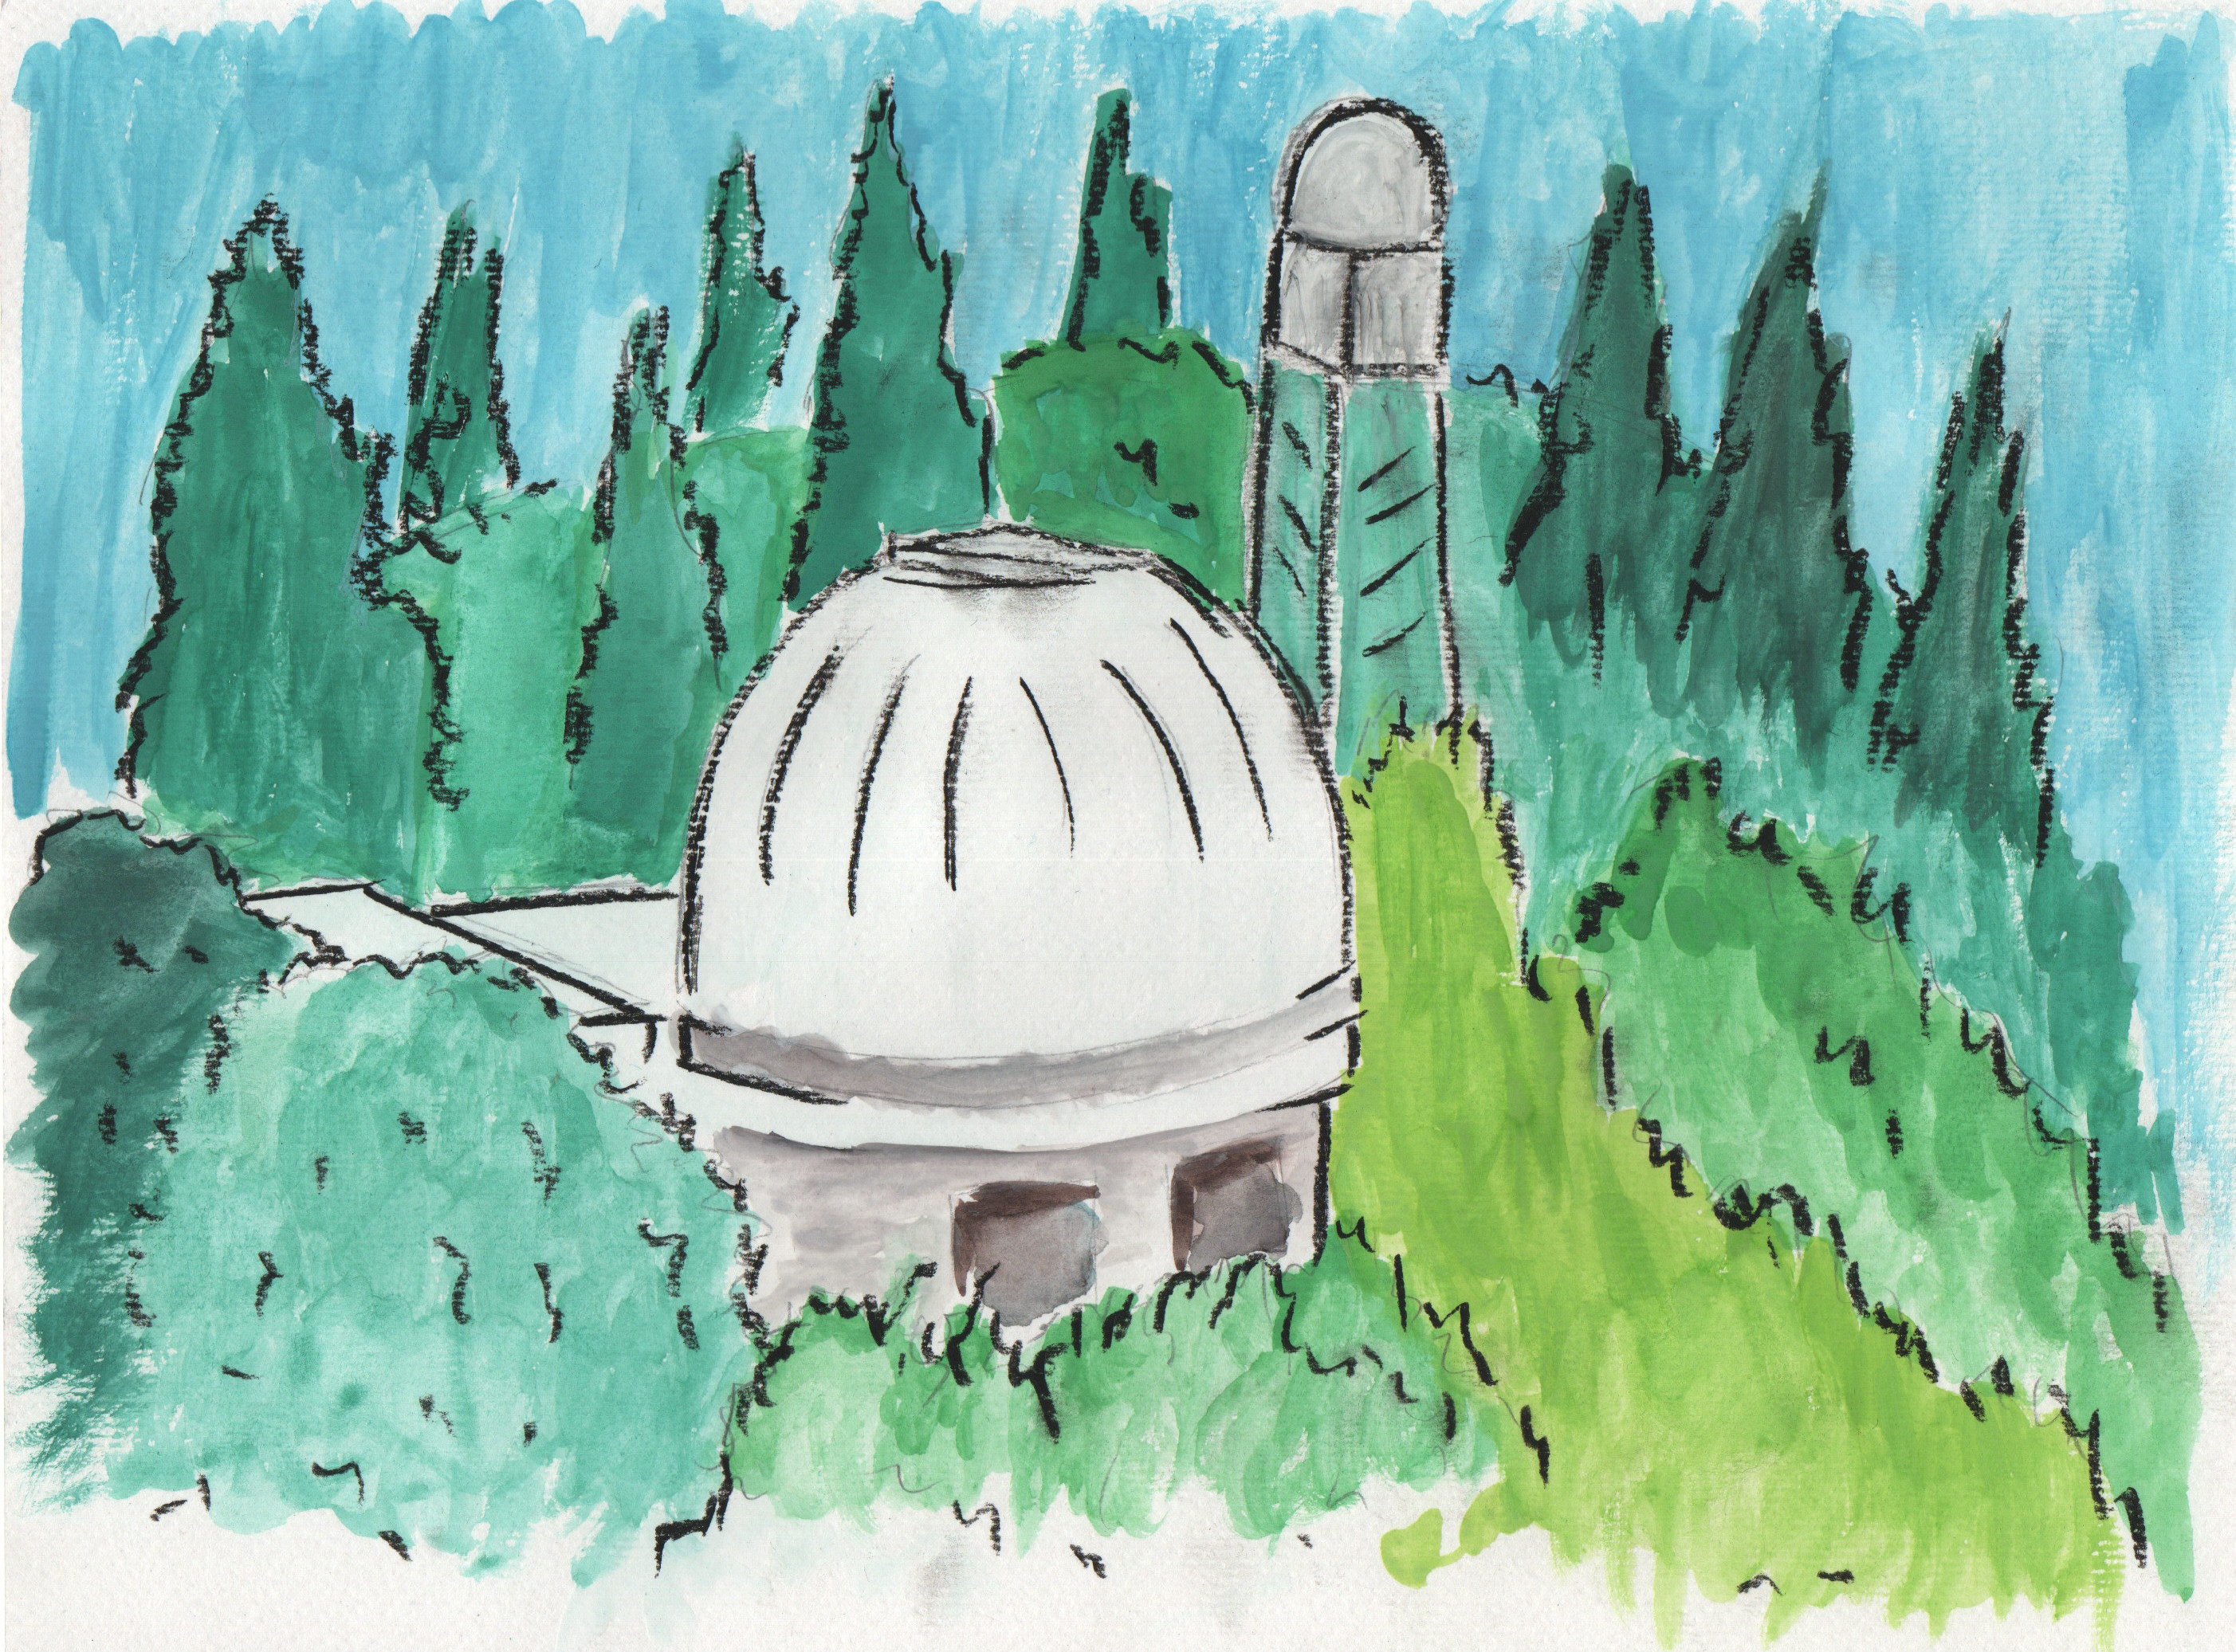
\includegraphics[width=26cm]{osservatorio_arcetri.jpg}};
			%\draw [ultra thick] (2,8) rectangle (28,-9.6);
			\draw [ultra thick, fill=dida] (1,14) rectangle (29,8);
			\node (example-textwidth-2) [right, align=left, text width=16cm, color=black, font=\fontsize{23pt}{24pt}\selectfont] at (11,11) {Preparando la tesi di laurea, ho lavorato a un piccolo telescopio di 30 cm di diametro, situato sul tetto dell'Osservatorio di Arcetri, sulle colline fiorentine, con la città distesa sotto.};
		\end{scope}
		% margherita hack
		\begin{scope}[shift={(0,3)}]
			\tkzDefPoint(6,0){M}
			\tkzDefPoint(1.5,0){R}
			\tkzDrawCircle[fill=earth,ultra thick](M,R)
			\node at (M) {
\includegraphics[width=8cm]{margherita_hack}};
		\end{scope}
		% osservatorio di notte
		\begin{scope}[shift={(0,-33)}]
			\node at (15,0) {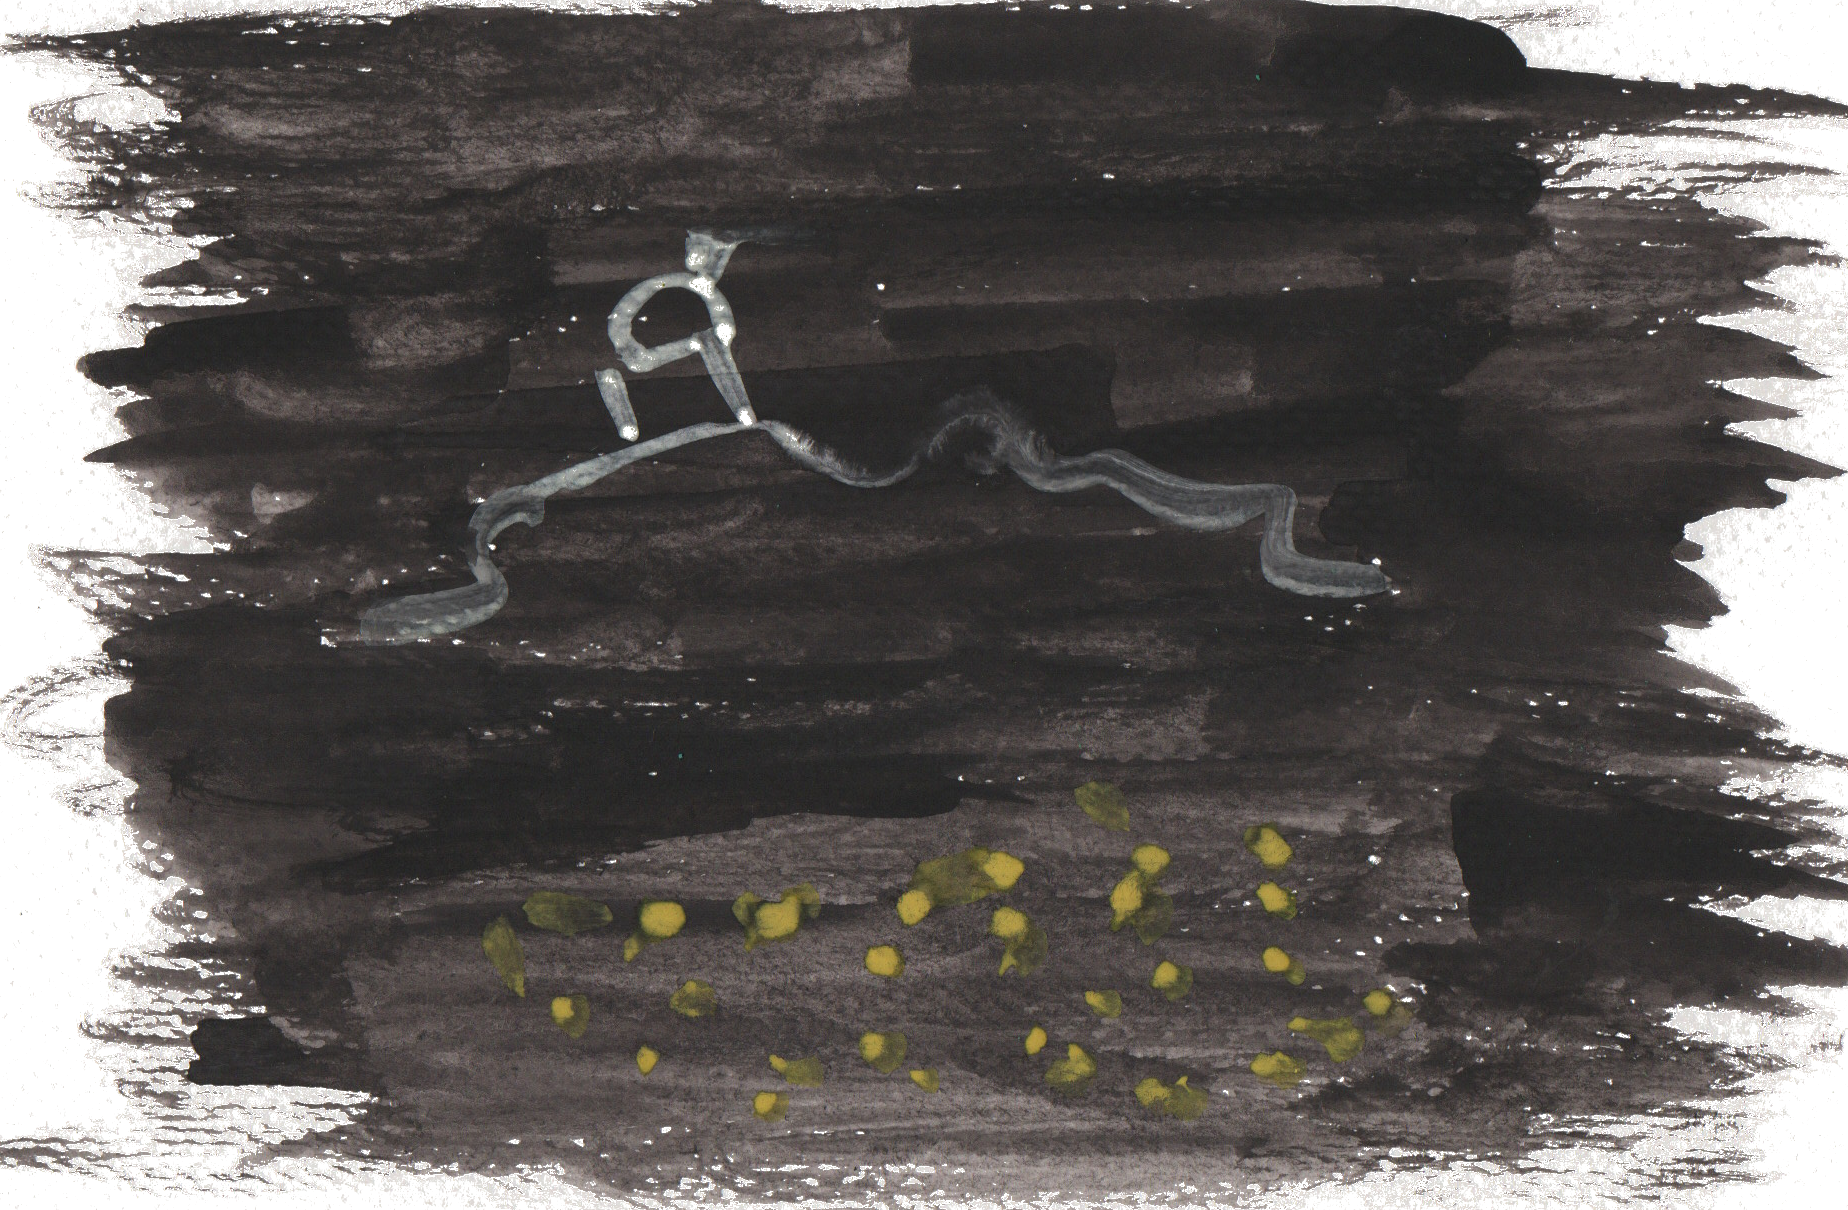
\includegraphics[width=26cm]{osservatorio_notte}};
			\draw [ultra thick, fill=dida] (1,16) rectangle (29,6);
			\node (example-textwidth-2) [right, align=left, text width=16cm, color=black, font=\fontsize{23pt}{24pt}\selectfont] at (2,11) {A quel tempo - era il 1944 - si potevano fare osservazioni, sebbene con uno strumento così modesto, ottenendo risultati degni d'essere pubblicati su riviste internazionali di grande prestigio. Allora non esisteva l'inquinamento luminoso, la guerra era in corso e le città sprofondavano nel buio più completo dell'oscuramento.};
		\end{scope}
		% telescopio
		\begin{scope}[shift={(0,-22)}]
			\tkzDefPoint(23,0){T}
			\tkzDefPoint(27.5,0){t}
			\tkzDrawCircle[fill=earth,ultra thick](T,t)
			\node at (T) {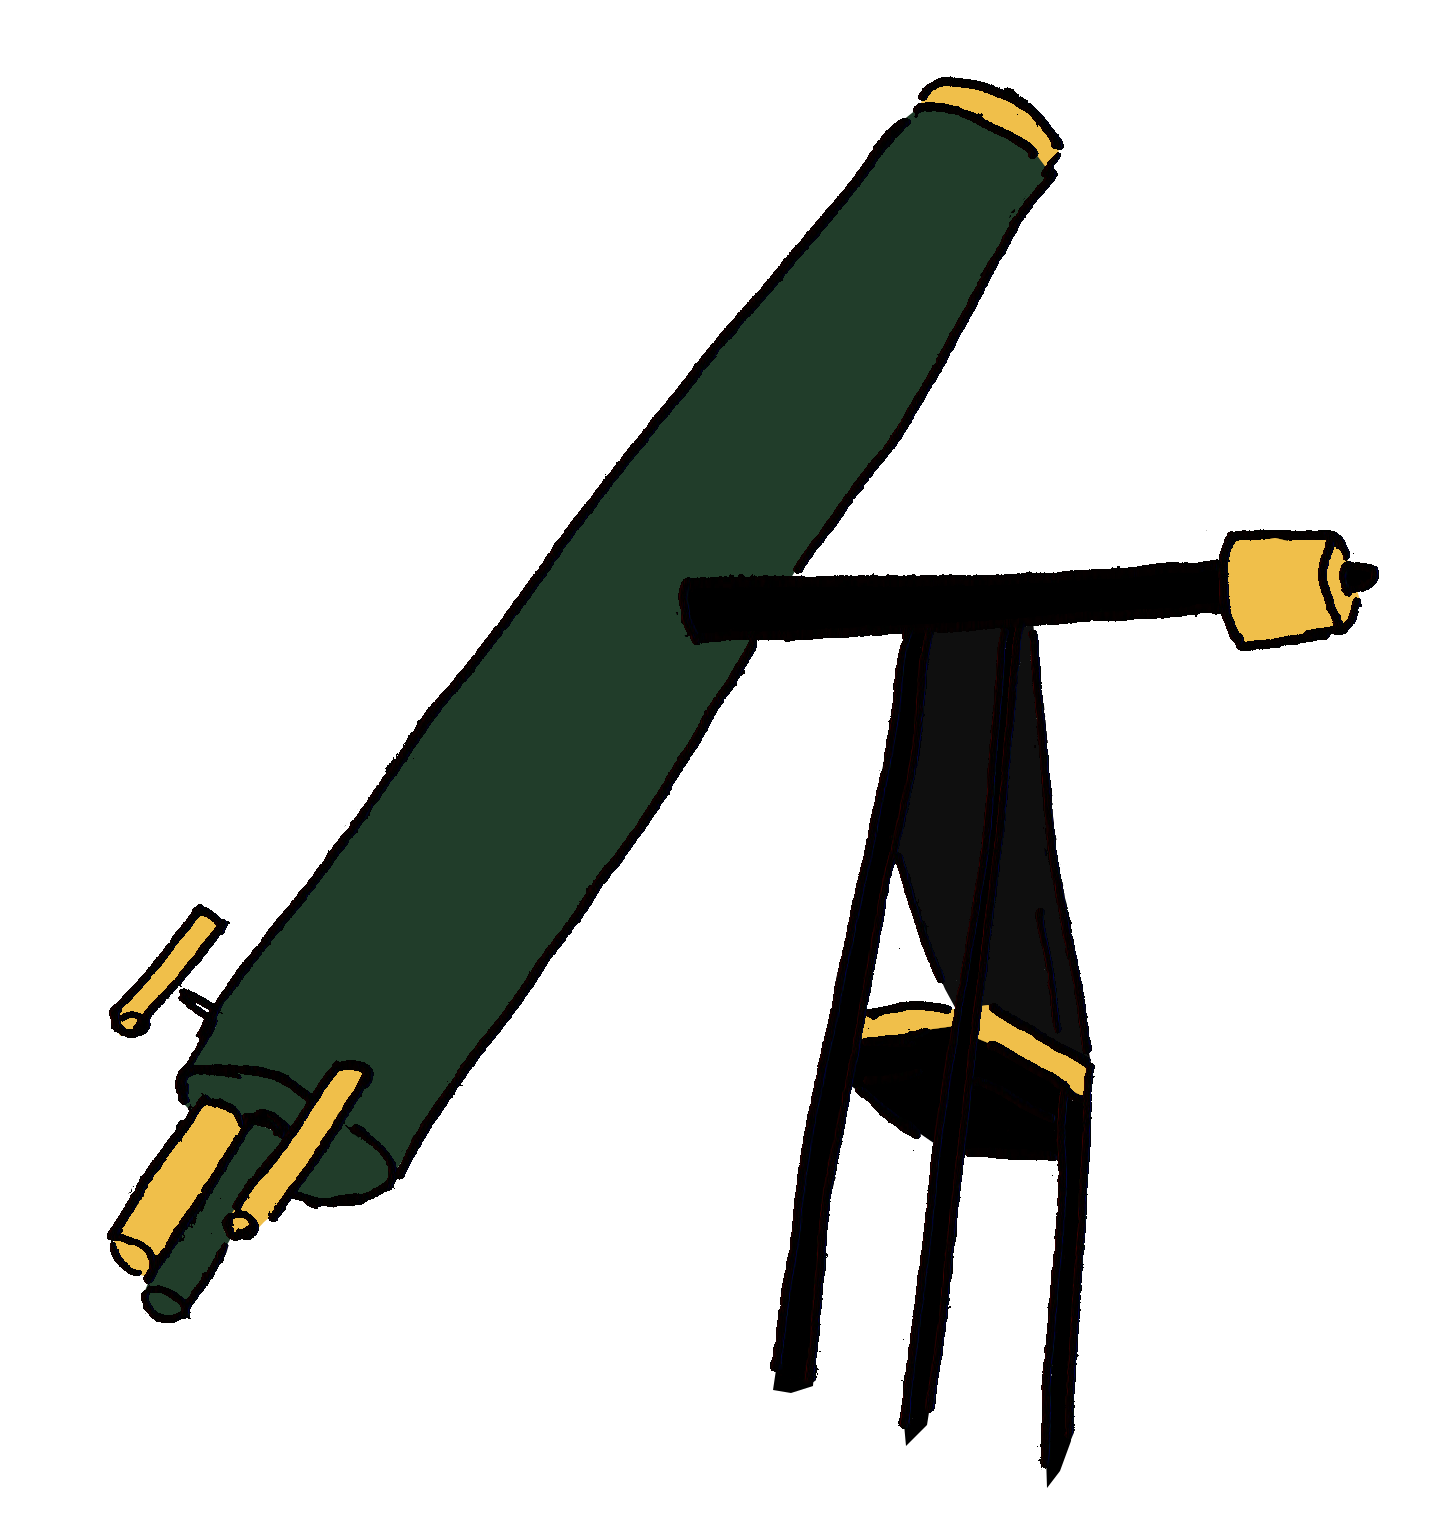
\includegraphics[width=7cm]{telescopio}};
		\end{scope}
		% merate
		\begin{scope}[shift={(0,-55)}]
			\node at (15,0) {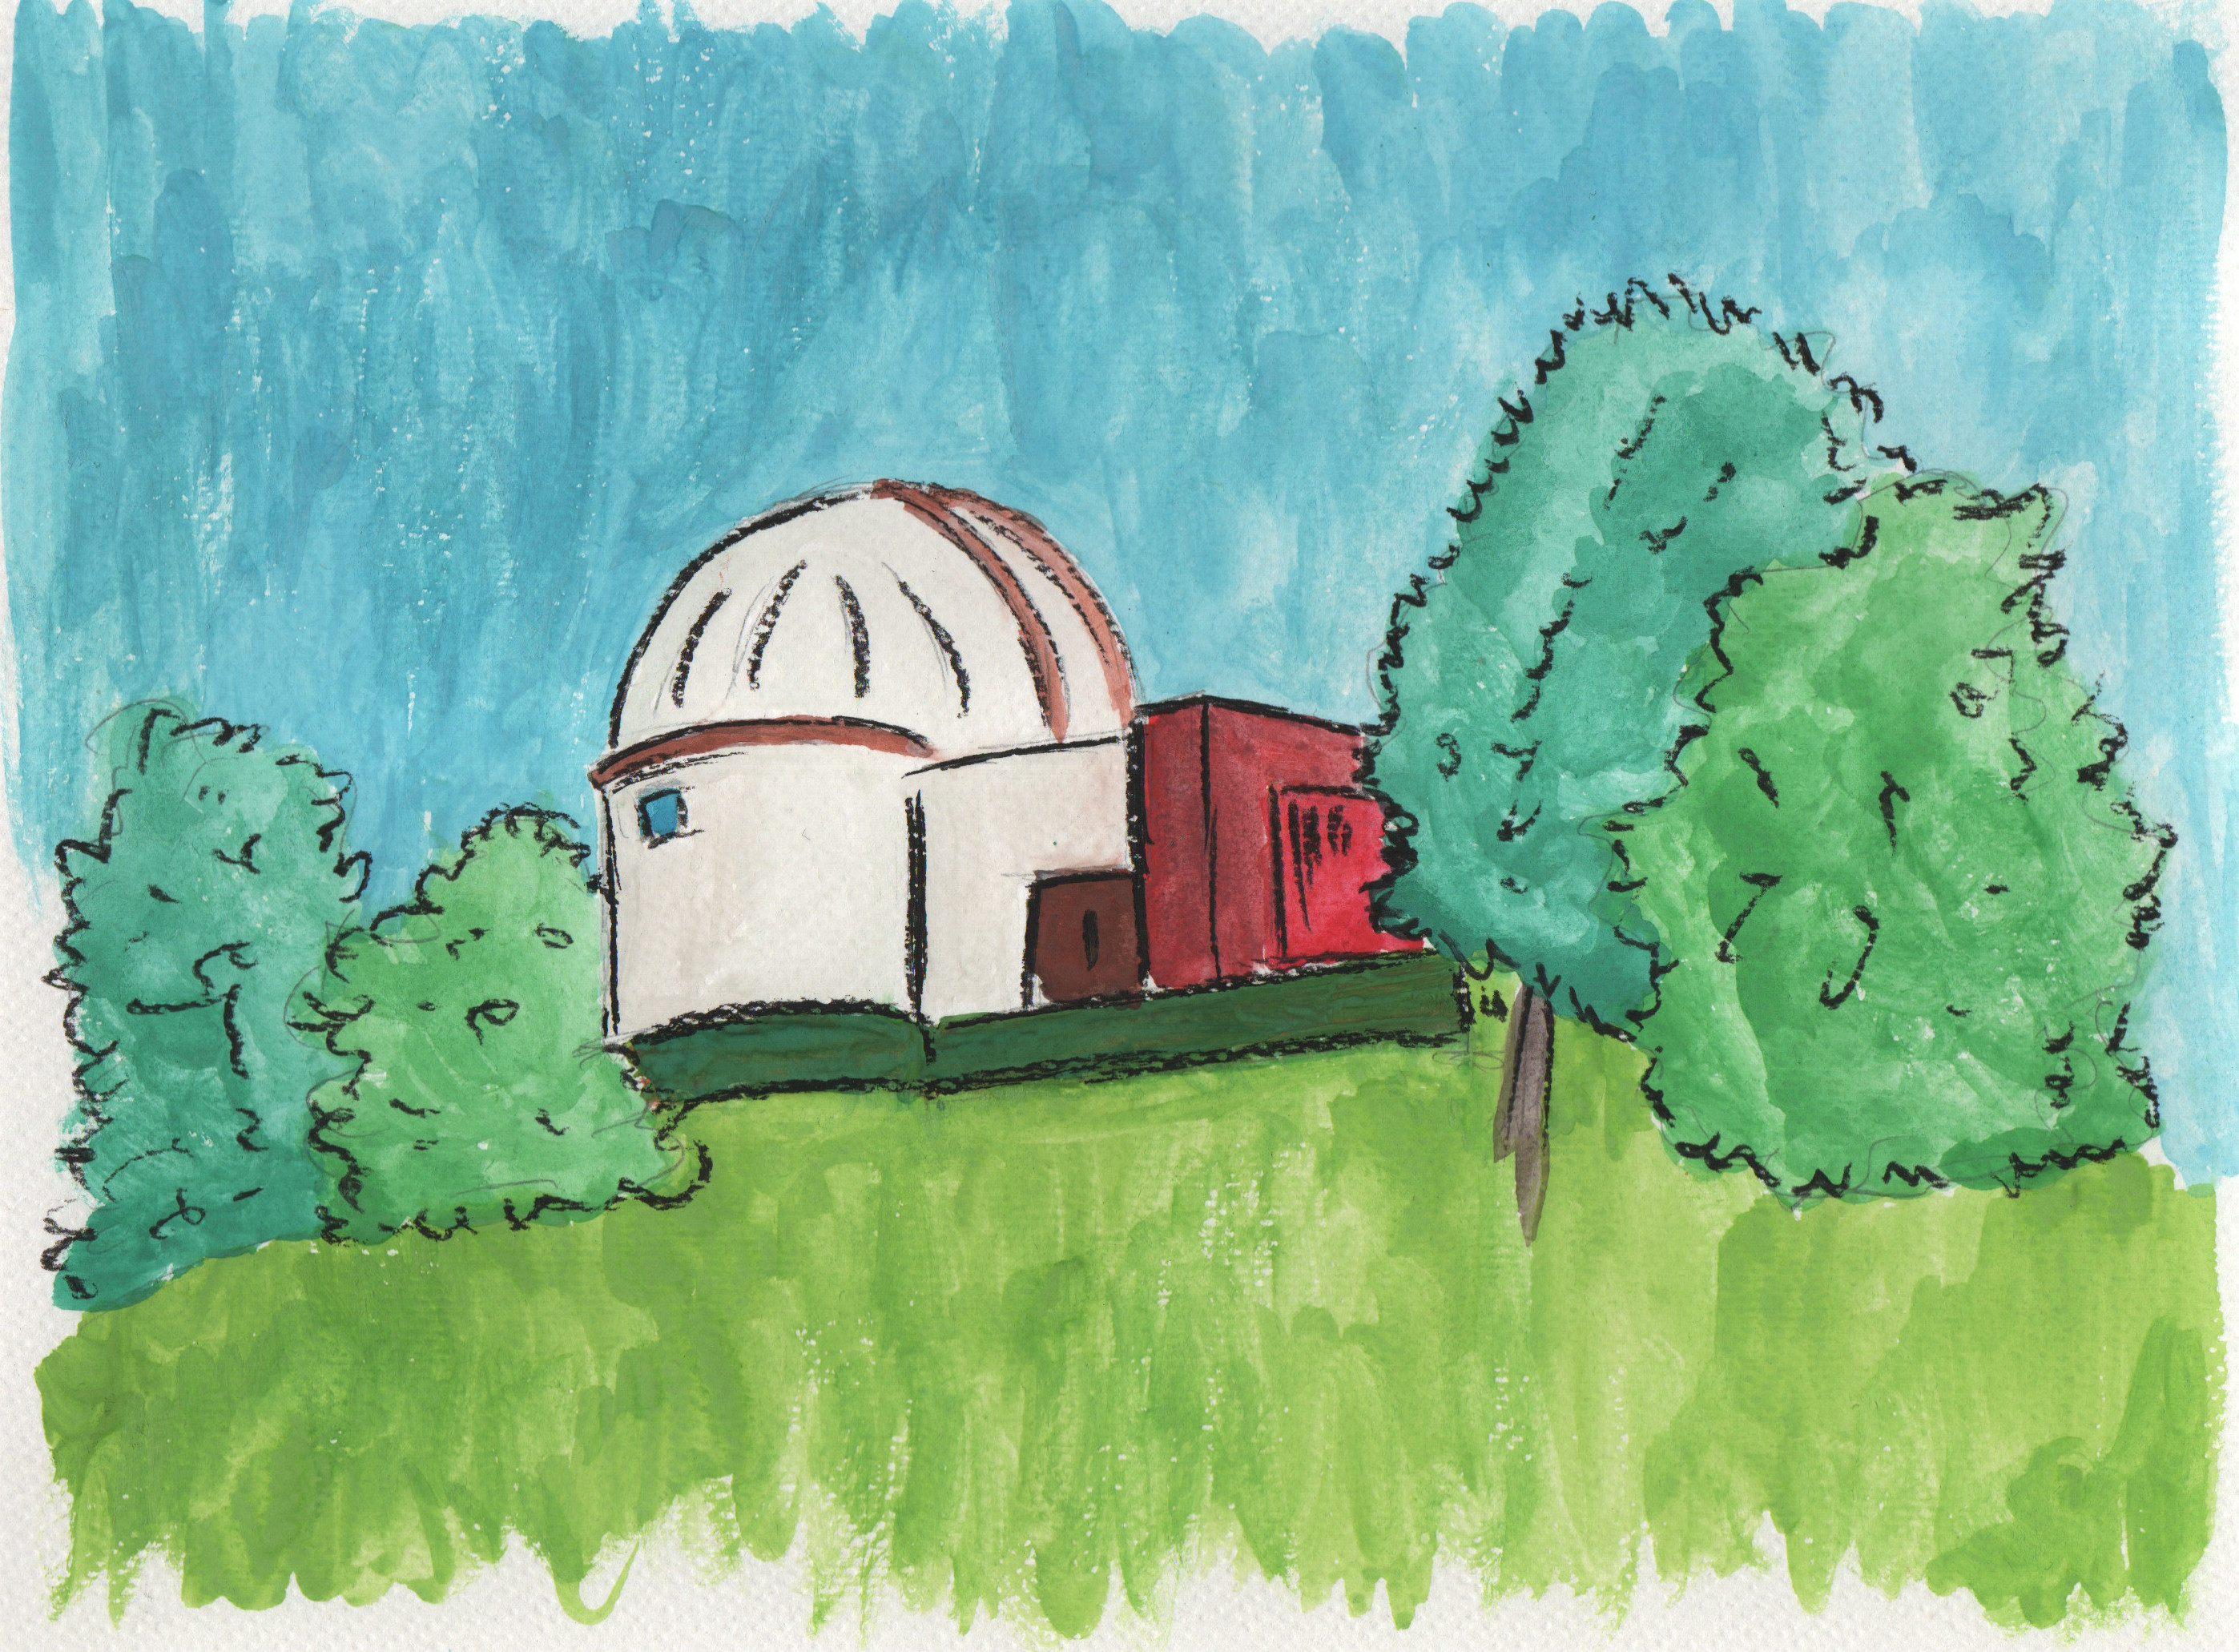
\includegraphics[width=26cm]{osservatorio_merate.jpg}};
			\draw [ultra thick, fill=dida] (1,14) rectangle (29,8);
			\node (example-textwidth-2) [right, align=left, text width=27cm, color=black, font=\fontsize{23pt}{24pt}\selectfont] at (1.5,11) {A Merate, succursale dell'Osservatorio di Brera a Milano, a soli 300 metri sul livello del mare, ho lavorato tutte le notti serene tra il '54 e il '64. Non era certo un posto ideale; in Brianza il cielo raramente è bello, quasi sempre velato da una leggera foschia. Solo dopo un temporale rimane terso per 2 o 3 giorni.};
		\end{scope}
		% merate foschia
		\begin{scope}[shift={(0,-77)}]
			\node at (15,0) {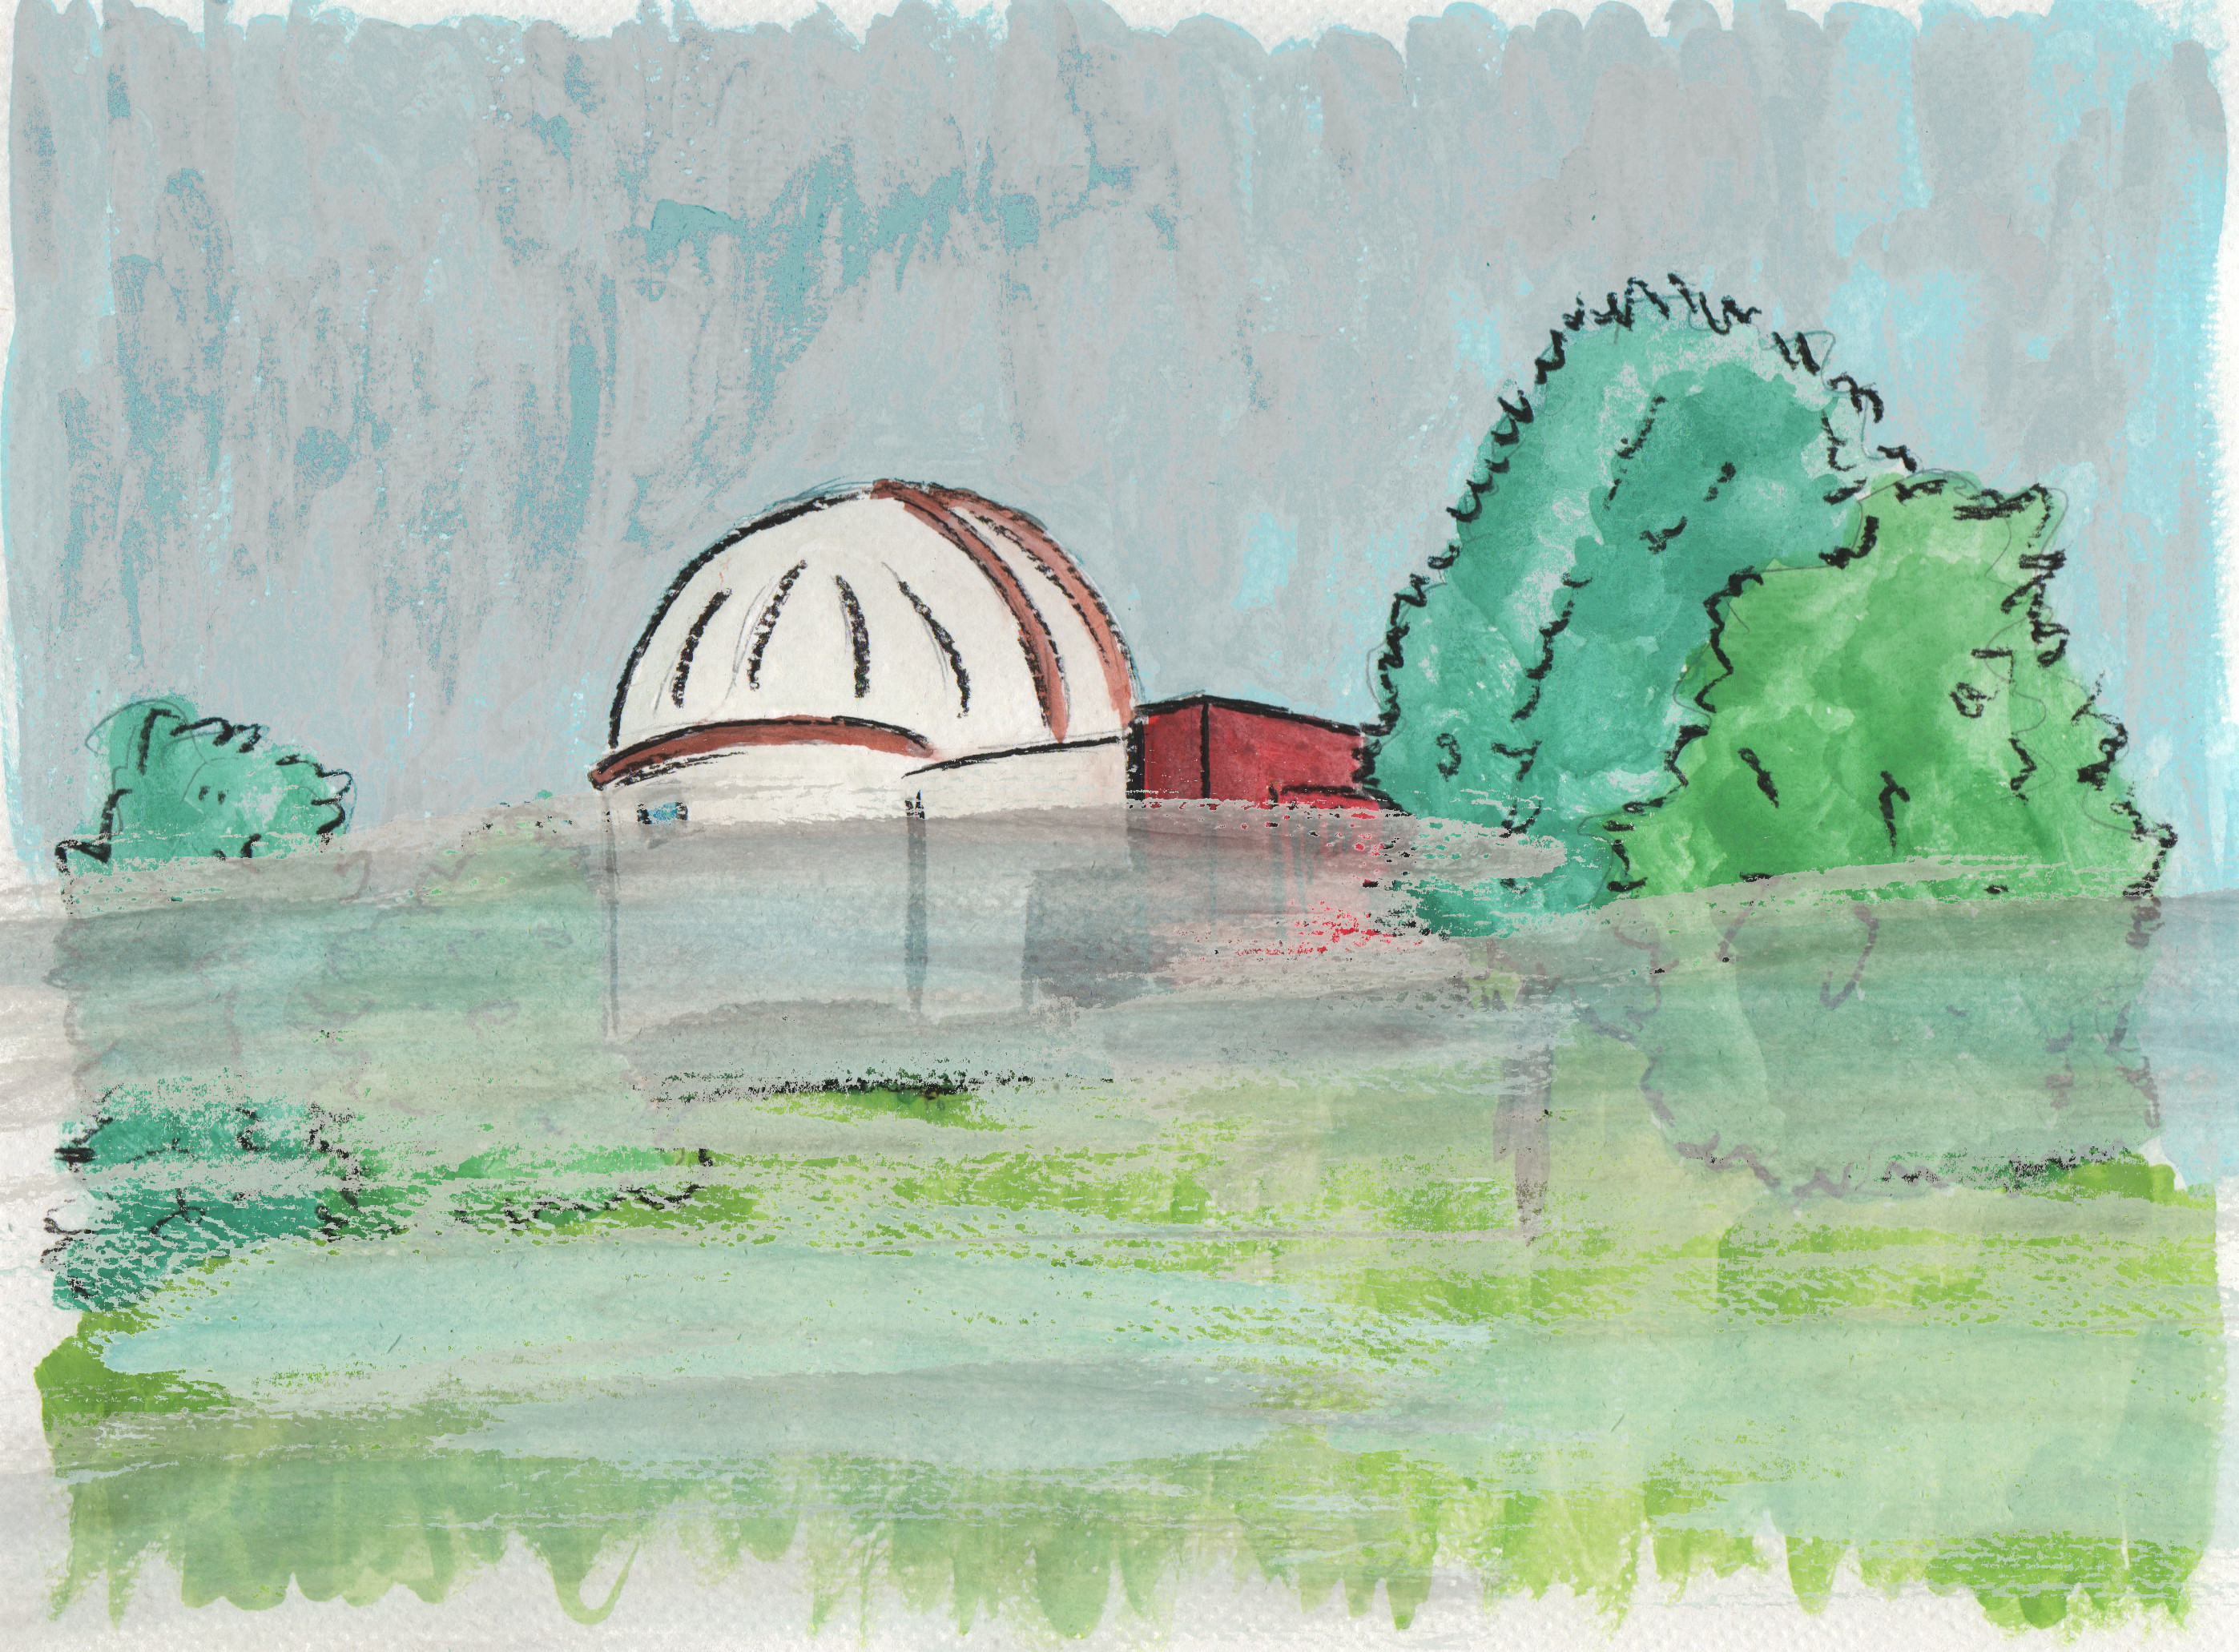
\includegraphics[width=26cm]{osservatorio_merate-foschia.jpg}};
			\draw [ultra thick, fill=dida] (1,14) rectangle (29,8);
			\node (example-textwidth-2) [right, align=left, text width=27cm, color=black, font=\fontsize{23pt}{24pt}\selectfont] at (1.5,11) {Le notti più limpide di solito capitano a settembre, dicembre e gennaio, poi la nebbia riduce molto lo splendore delle stelle. A Merate la cupola del telescopio Zeiss è su una collinetta che sovrasta di una decina di metri il parco sottostante. Spesso la cupola emergeva a mala pena dalla nebbia.};
		\end{scope}
		% moon with skyline
		\begin{scope}[shift={(0,-98)}]
			\draw [fill=space] (-1,9) rectangle (31,-11);
			%moon
			\tkzDefPoint(15,-0.2){L}
			\tkzDefPoint(6.2,0){L1}
			\tkzDefShiftPoint[L1](0:17.6){La1}
			\tkzDefShiftPoint[L1](0:17.55){La2}
			\tkzDrawCircle[color=moon,fill=moon,ultra thick](L,L1)
			\tkzDrawArc[ultra thick, rotate](L,La1)(-80)
			\tkzDrawArc[ultra thick, rotate](L,La1)(80)
			\tkzDrawArc[ultra thick, rotate](L,La2)(-78)
			\tkzDrawArc[ultra thick, rotate](L,La2)(78)
			%
			\tkzDefPoint(15.5,-6.2){C3}
			\tkzDefShiftPoint[C3](0:0.3){Cr3}
			\tkzDefShiftPoint[Cr3](0:-0.05){Ca3}
			\tkzDrawArc[thick, color=linem, rotate](L,C3)(-15)
			\tkzDrawArc[thick, color=linem, rotate](L,C3)(15)
			\tkzDrawArc[rotate around={10:(C3)},thick, color=linem, rotate](L,C3)(-10)
			\tkzDrawArc[rotate around={10:(C3)},thick, color=linem, rotate](L,C3)(10)
			\tkzDrawArc[rotate around={-10:(C3)},thick, color=linem, rotate](L,C3)(-10)
			\tkzDrawArc[rotate around={-10:(C3)},thick, color=linem, rotate](L,C3)(10)
			\begin{scope}[yscale=0.8]
				\tkzDrawCircle[color=linem,fill=linem](C3,Cr3)
				\tkzDrawArc[rotate around={30:(C3)},rotate](C3,Ca3)(30)
			\end{scope}
			%
			\tkzDefPoint(7.4,-3.6){M1}
			\tkzDefShiftPoint[M1](0:0.15){Mr1}
			\tkzDefShiftPoint[Mr1](0:-0.05){Ma1}
			\begin{scope}[rotate around={30:(M1)},yscale=1.8]
				\tkzDrawCircle[color=craterm,fill=craterm](M1,Mr1)
				\tkzDrawArc[rotate around={220:(M1)},thick,color=linem,rotate](M1,Ma1)(40)
			\end{scope}
			%
			\tkzDefPoint(20.8,4.7){M2}
			\tkzDefShiftPoint[M2](0:0.7){Mr2}
			\tkzDefShiftPoint[Mr2](0:-0.1){Ma2}
			\begin{scope}[rotate around={40:(M2)},yscale=1.9]
				\tkzDrawCircle[color=craterm,fill=craterm](M2,Mr2)
				\tkzDrawArc[rotate around={-10:(M2)},thick,color=linem,rotate](M2,Ma2)(40)
			\end{scope}
			%
			\tkzDefPoint(15.8,4.6){M3}
			\tkzDefShiftPoint[M3](0:1.5){Mr3}
			\tkzDefShiftPoint[Mr3](0:-0.1){Ma3}
			\begin{scope}[yscale=0.8]
				\tkzDrawCircle[color=craterm,fill=craterm](M3,Mr3)
				\tkzDrawArc[rotate around={30:(M3)},thick,color=linem,rotate](M3,Ma3)(40)
			\end{scope}
			%
			\tkzDefPoint(18.1,2.8){M4}
			\tkzDefShiftPoint[M4](0:1.5){Mr4}
			\tkzDefShiftPoint[Mr4](0:-0.1){Ma4}
			\begin{scope}[rotate around={20:(M4)},yscale=1.1]
				\tkzDrawCircle[color=craterm,fill=craterm](M4,Mr4)
				\tkzDrawArc[rotate around={20:(M4)},thick,color=linem,rotate](M4,Ma4)(40)
			\end{scope}
			%
			\tkzDefPoint(22.5,1.3){C2}
			\tkzDefPoint(21,1.9){M5}
			\tkzDefShiftPoint[M5](0:1.3){Mr5}
			\begin{scope}[rotate around={42:(M5)},yscale=2]
				\tkzDrawCircle[color=craterm,fill=craterm](M5,Mr5)
				\tkzDrawArc[thick,color=linem,rotate](M5,C2)(40)
				\tkzDrawArc[thick,color=linem,rotate](M5,C2)(-40)
			\end{scope}
			%
			\tkzDefPoint(9.2,0.2){M6}
			\tkzDefShiftPoint[M6](0:3){Mr6}
			\tkzDefShiftPoint[Mr6](0:-0.1){Ma6}
			\begin{scope}[yscale=1.4]
				\tkzDrawCircle[color=craterm,fill=craterm](M6,Mr6)
				\tkzDrawArc[rotate around={-160:(M6)},thick,color=linem,rotate](M6,Ma6)(40)
			\end{scope}
			%
			\tkzDefPoint(11,3.4){M7}
			\tkzDefShiftPoint[M7](0:2){Mr7}
			\tkzDefShiftPoint[Mr7](0:-0.1){Ma7}
			\begin{scope}[rotate around={-20:(M7)},yscale=1.3]
				\tkzDrawCircle[color=craterm,fill=craterm](M7,Mr7)
				\tkzDrawArc[rotate around={30:(M7)},thick,color=linem,rotate](M7,Ma7)(40)
			\end{scope}
			%
			\tkzDefPoint(11.2,0.5){C1}
			\tkzDefShiftPoint[C1](0:0.2){Cr1}
			\tkzDefShiftPoint[Cr1](0:-0.05){Ca1}
			\tkzDrawCircle[color=linem,fill=linem](C1,Cr1)
			\tkzDrawArc[rotate around={30:(C1)},rotate](C1,Ca1)(50)
			%
			\tkzDefShiftPoint[C2](0:0.2){Cr2}
			\tkzDefShiftPoint[Cr2](0:-0.05){Ca2}
			\begin{scope}[yscale=1.4]
				\tkzDrawCircle[color=linem,fill=linem](C2,Cr2)
				\tkzDrawArc[rotate around={20:(C2)},rotate](C2,Ca2)(40)
			\end{scope}
			%
			\tkzDefPoint(9.1,-0.5){C4}
			\tkzDefShiftPoint[C4](0:0.05){Cr4}
			\begin{scope}[yscale=1.1]
				\tkzDrawCircle[color=linem,fill=linem](C4,Cr4)
			\end{scope}
			% skyline
			\begin{scope}[shift={(0,-8)}]
				\tkzDefPoint(-2,-3){S1}
				\tkzDefPoint(0,4){S2}
				\tkzDefPoint(1.5,3){S3}
				\tkzDefPoint(3,5){S4}
				\tkzDefPoint(5,0){S5}
				\tkzDefPoint(7,4){S6}
				\tkzDefPoint(10,2){S7}
				\tkzDefPoint(11,3){S8}
				\tkzDefPoint(13,-2){S9}
				\tkzDefPoint(15,0){S10}
				\tkzDefPoint(19,-2){S11}
				%
				\tkzDefPoint(24,-2){S12}
				\tkzDefPoint(24,-1){S13}
				\tkzDefPoint(23.5,-1){S14}
				\tkzDefPoint(25,0){S15}
				\tkzDefPoint(27,-1){S16}
				\tkzDefPoint(26.5,-1){S17}
				\tkzDefPoint(26.5,-2){S18}
				\tkzDefPoint(28,-2){S19}
				\tkzDefPoint(30,-3){S20}
				\tkzDrawPolygon[fill=black](S1,S2,S3,S4,S5,S6,S7,S8,S10,S11,S12,S13,S14,S15,S16,S17,S18,S19,S20)
			\end{scope}
		\end{scope}
		% dida skyline
		\begin{scope}[shift={(0,-99)}]
			\draw [ultra thick, fill=dida] (1,14) rectangle (29,8);
			\node (example-textwidth-2) [right, align=left, text width=27cm, color=black, font=\fontsize{23pt}{24pt}\selectfont] at (1.5,11) {Nei quindici giorni delle fasi lunari tra il primo e l'ultimo quarto, che comprendeva dunque la Luna piena, si lavorava con lo spettrografo. L'immagine della stella cadeva su una sottile fenditura e perciò il chiarore del cielo illuminato dalla Luna non dava nessun disturbo.};
		\end{scope}
		% fotometristi
		\begin{scope}[shift={(0,-118)}]
			\node at (7,0) {
\includegraphics[width=10cm]{fotometristi}};
			\node (example-textwidth-2) [notice={(-3,0.5)}, ultra thick, right, align=center, text width=12cm, color=black, fill=white, font=\fontsize{23pt}{24pt}\selectfont] at (12,-1) {La Luna non c'è... Possiamo uscire, Padrone!};
			\draw [ultra thick, fill=dida] (2.4,-5) rectangle (12,-8);
			\node (example-textwidth-2) [right, align=center, text width=10cm, color=black, font=\fontsize{20pt}{21pt}\selectfont] at (2,-6.5) {Fotometristi dopo all'incirca tre settimane di luce lunare.};
		\end{scope}
		% fotometristi dida
		\begin{scope}[shift={(0,-121.5)}]
			\draw [ultra thick, fill=dida] (1,13) rectangle (29,9);
			\node (example-textwidth-2) [right, align=left, text width=27cm, color=black, font=\fontsize{23pt}{24pt}\selectfont] at (1.5,11) {Nei quindici giorni fra l'ultimo e il primo quarto, includenti la Luna nuova, lavoravano i fotometristi che avevano bisogno di un cielo quanto più scuro possibile.};
		\end{scope}
		%
		\begin{scope}[shift={(0,-127)}]
			\node at (27,0) () {
\includegraphics[width=3.7cm]{licenza}};
			\node at (21.7,0.5) {\textcolor{black}{\fontsize{14}{15}\selectfont Testo: Margherita Hack}};
			\node at (19,0) {\textcolor{black}{\fontsize{14}{15}\selectfont Illustrazioni: @ulaulaman - Gianluigi Filippelli}};
			\node at (19.4,-0.5) {\textcolor{black}{\fontsize{14}{15}\selectfont La licenza è relativa solo alle illustrazioni}};
		\end{scope}
	\end{tikzpicture}
%
\end{document}